% Il blocco tratteggiato è ripetuto in sequenza, non in parallelo.
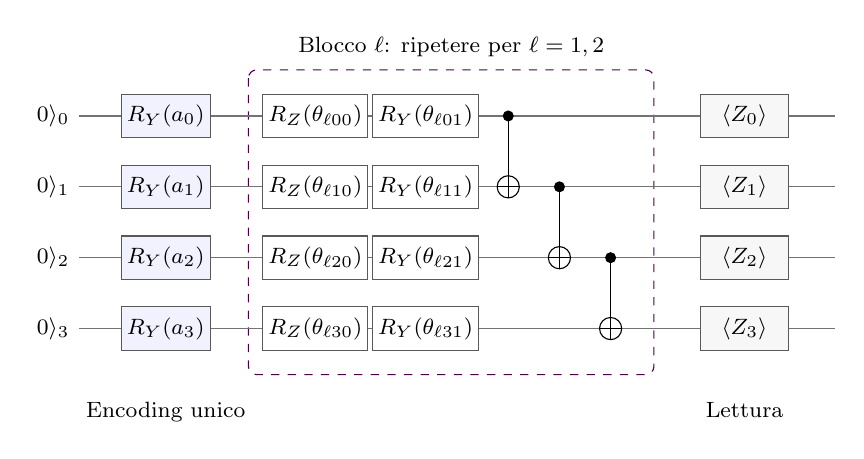
\begin{tikzpicture}[
  x=1cm,y=0.9cm,font=\footnotesize,
  gate/.style={draw=black!65,fill=white,minimum height=0.55cm,
    minimum width=1.12cm,inner sep=2pt}
]
\draw[dashed,rounded corners=3pt,draw=violet!60!black]
  (2.15,0.65) rectangle (7.3,-3.65);
\node[anchor=south,align=center] at (4.725,0.7)
  {Blocco \(\ell\): ripetere per \(\ell=1,2\)};
\foreach \j in {0,1,2,3}{
  \draw[black!55] (0,-\j) -- (9.6,-\j);
  \node[anchor=east] at (0,-\j) {\(\lvert0\rangle_{\j}\)};
  \node[gate,fill=blue!5] at (1.1,-\j) {\(R_Y(a_{\j})\)};
  \node[gate] at (3,-\j) {\(R_Z(\theta_{\ell\j0})\)};
  \node[gate] at (4.4,-\j) {\(R_Y(\theta_{\ell\j1})\)};
  \node[gate,fill=black!3] at (8.45,-\j) {\(\langle Z_{\j}\rangle\)};
}
\foreach \x/\control/\target in {5.45/0/1,6.1/1/2,6.75/2/3}{
  \draw (\x,-\control) -- (\x,-\target);
  \fill (\x,-\control) circle (2pt);
  \draw[fill=white] (\x,-\target) circle (4pt);
  \draw (\x-0.14,-\target) -- (\x+0.14,-\target);
  \draw (\x,-\target-0.155) -- (\x,-\target+0.155);
}
\node[anchor=north] at (1.1,-3.9) {Encoding unico};
\node[anchor=north] at (8.45,-3.9) {Lettura};
\end{tikzpicture}
